\documentclass[12pt,letterpaper]{article}

% Packages
\usepackage[utf8]{inputenc}
\usepackage[margin=1in]{geometry}
\usepackage{amsmath,amssymb,amsthm}
\usepackage{graphicx}
\usepackage{bm}
\usepackage{hyperref}
\usepackage{cite}
\usepackage{float}
\usepackage{enumitem}
\usepackage{algorithm}
\usepackage{algpseudocode}
\usepackage{listings}
\usepackage{xcolor}
\usepackage{tikz}
\usetikzlibrary{arrows.meta,positioning,calc,shapes.geometric}

% Code listing style
\lstset{
    basicstyle=\ttfamily\small,
    keywordstyle=\color{blue},
    commentstyle=\color{green!60!black},
    stringstyle=\color{red},
    showstringspaces=false,
    breaklines=true,
    frame=single,
    numbers=left,
    numberstyle=\tiny\color{gray}
}

% Math commands
\newcommand{\vect}[1]{\bm{#1}}
\newcommand{\mat}[1]{\bm{#1}}

% Title
\title{\textbf{Hierarchical Control Architecture for Fixed-Wing Aircraft:\\A Multi-Level Cascaded Approach}}
\author{Technical Documentation\\
\small Inspired by dRehmFlight (Nicholas Rehm)}
\date{\today}

\begin{document}

\maketitle

\begin{abstract}
This document presents a comprehensive five-level hierarchical control architecture for fixed-wing aircraft, designed for autonomous flight, reinforcement learning research, and flight control education. The architecture implements a cascaded control structure that separates high-level mission planning from low-level actuation, enabling flexible agent design at multiple abstraction levels. The core design---separating attitude (angle mode) from rate (acro mode) control---is directly inspired by dRehmFlight \cite{rehm_drehm}, a widely-used open-source flight controller by Nicholas Rehm. We extend this proven architecture with additional high-level layers (waypoint navigation, HSA control) and provide rigorous mathematical foundations suitable for graduate-level study. The system combines Python flexibility for high-level control with C++ performance for time-critical inner loops, achieving real-time performance suitable for both simulation and hardware deployment.
\end{abstract}

\tableofcontents
\newpage

% ============================================================================
\section{Introduction}
% ============================================================================

\subsection{Motivation and Background}

Aircraft control is inherently hierarchical. A pilot does not directly think about aileron deflection angles when commanding a turn; instead, they think in terms of desired bank angles, headings, or waypoints. This natural abstraction hierarchy has been formalized in modern flight control systems through \textbf{cascaded control architectures}.

The challenge in autonomous aircraft control is to bridge the gap between high-level mission objectives (e.g., ``fly to waypoint at 100m altitude'') and low-level actuator commands (e.g., ``set aileron to -0.3 radians''). A well-designed control hierarchy:

\begin{enumerate}[noitemsep]
    \item \textbf{Separates concerns}: Each level addresses a specific abstraction
    \item \textbf{Enables modularity}: Levels can be swapped or improved independently
    \item \textbf{Facilitates learning}: Agents can operate at any level appropriate to their task
    \item \textbf{Provides robustness}: Outer loops handle disturbances, inner loops ensure tight tracking
    \item \textbf{Matches hardware realities}: Fast inner loops run on dedicated hardware, slower outer loops on general-purpose processors
\end{enumerate}

\subsection{Inspiration from dRehmFlight}

This control architecture is fundamentally inspired by \textbf{dRehmFlight} \cite{rehm_drehm}, an open-source flight controller developed by Nicholas Rehm for small fixed-wing and multirotor aircraft. dRehmFlight pioneered an accessible yet rigorous approach to cascaded flight control, clearly separating:

\begin{itemize}[noitemsep]
    \item \textbf{Angle mode (stabilized)}: Outer loop controls Euler angles, outputs rate commands
    \item \textbf{Rate mode (acro)}: Inner loop controls angular rates, outputs surface deflections
\end{itemize}

This separation---which we adopt as Levels 3 and 4 in our architecture---is the foundation of virtually all modern flight controllers, including Betaflight \cite{betaflight}, ArduPilot \cite{ardupilot}, and PX4 \cite{px4}. dRehmFlight's clear pedagogical presentation and well-documented design patterns make it an ideal reference for understanding cascaded control.

\textbf{Our contribution} extends dRehmFlight's core two-loop structure by adding:
\begin{itemize}[noitemsep]
    \item \textbf{Level 2 (HSA --- Heading, Speed, Altitude)}: Control for autonomous flight
    \item \textbf{Level 1 (Waypoint)}: 3D navigation with guidance algorithms
    \item \textbf{Level 5 (Surface)}: Explicit surface control layer for RL research
    \item \textbf{Mathematical rigor}: Graduate-level derivations of control laws
    \item \textbf{Python/C++ hybrid}: Flexibility for research with performance for deployment
\end{itemize}

While our implementation is original, the conceptual design and control philosophy owe a significant debt to dRehmFlight's proven architecture.

\subsection{Document Organization}

This document is structured bottom-up, starting with the innermost (fastest) control loop and progressing outward:

\begin{itemize}[noitemsep]
    \item \textbf{Section 2}: Overview of 5-level hierarchy
    \item \textbf{Section 3}: Level 4 (Rate control) --- the critical inner loop
    \item \textbf{Section 4}: Level 3 (Attitude control) --- cascaded outer loop
    \item \textbf{Section 5}: Level 2 (HSA control) --- flight state tracking
    \item \textbf{Section 6}: Level 1 (Waypoint navigation) --- mission-level guidance
    \item \textbf{Section 7}: Level 5 (Direct surface control) --- for advanced research
    \item \textbf{Section 8}: Mathematical foundations (frequency domain, stability)
    \item \textbf{Section 9}: Implementation details (software, real-time)
    \item \textbf{Section 10}: Comparison to industry standards
\end{itemize}

% ============================================================================
\section{Control Hierarchy Overview}
% ============================================================================

\subsection{The Five Control Levels}

The architecture consists of five hierarchical control levels, each providing a different abstraction:

\begin{table}[H]
\centering
\caption{Five-Level Control Hierarchy}
\label{tab:levels}
\begin{tabular}{|c|l|l|l|}
\hline
\textbf{Level} & \textbf{Name} & \textbf{Input} & \textbf{Output} \\
\hline
1 & Waypoint Navigation & 3D position (N, E, D) & HSA command \\
2 & HSA Control & Heading, Speed, Altitude & Attitude angles \\
3 & Attitude Control & Roll, Pitch, Yaw angles & Angular rates \\
4 & Rate Control & Angular rates (p, q, r) & Surface deflections \\
5 & Surface Control & Surface deflections & Actuator commands \\
\hline
\end{tabular}
\end{table}

\subsection{Cascaded Control Flow}

The control flow propagates through the hierarchy:

\begin{equation}
\text{Waypoint} \xrightarrow{\text{L1}} \text{HSA} \xrightarrow{\text{L2}} \text{Attitude} \xrightarrow{\text{L3}} \text{Rates} \xrightarrow{\text{L4}} \text{Surfaces} \xrightarrow{\text{L5}} \text{Aircraft}
\end{equation}

\begin{figure}[H]
\centering
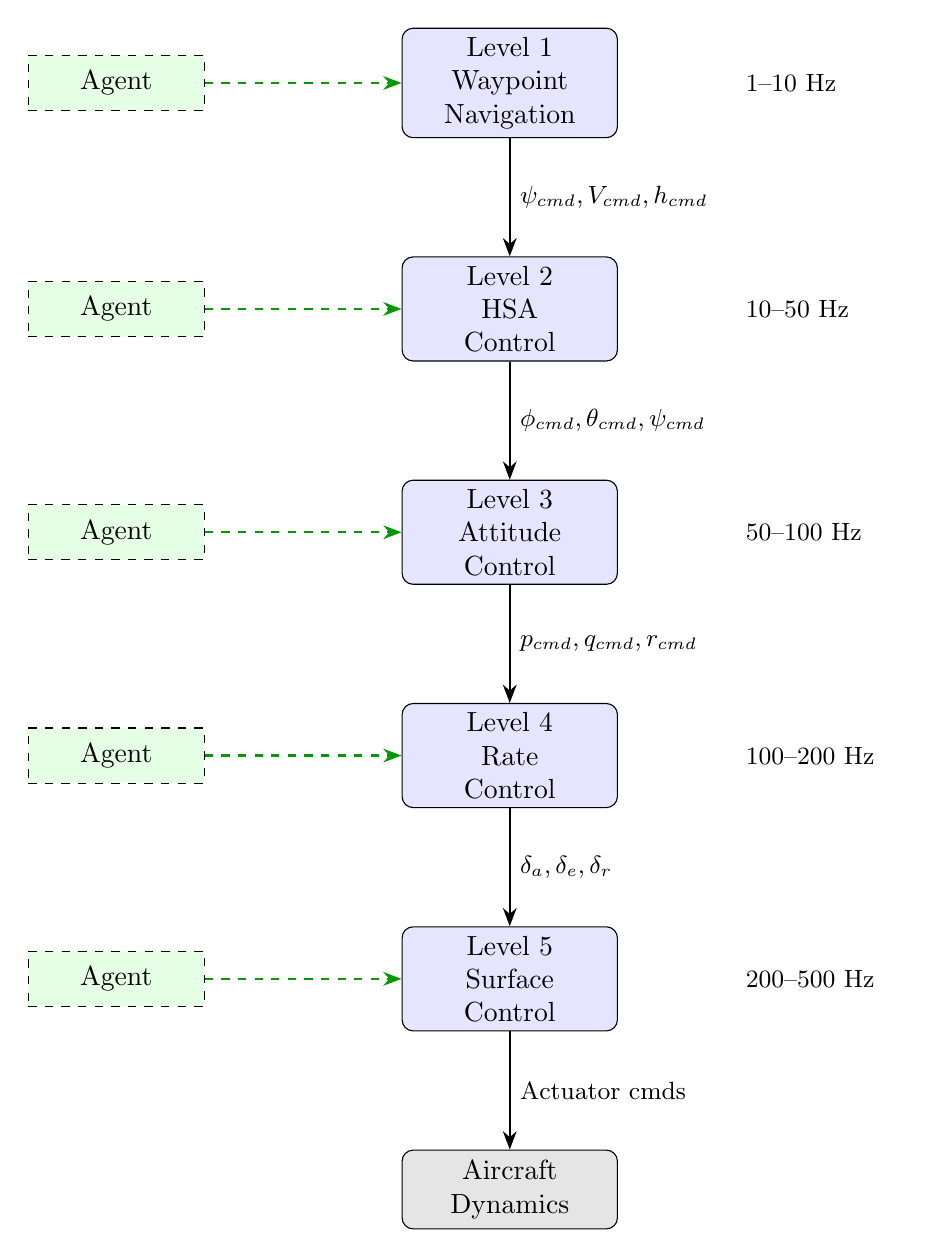
\begin{tikzpicture}[
    node distance=1.5cm,
    box/.style={rectangle, draw, fill=blue!10, text width=2.5cm, align=center, minimum height=1cm, rounded corners},
    agent/.style={rectangle, draw, fill=green!10, text width=2cm, align=center, minimum height=0.7cm, dashed},
    arrow/.style={-Stealth, thick}
]
    % Level boxes
    \node[box] (l1) {Level 1\\Waypoint\\Navigation};
    \node[box, below=of l1] (l2) {Level 2\\HSA\\Control};
    \node[box, below=of l2] (l3) {Level 3\\Attitude\\Control};
    \node[box, below=of l3] (l4) {Level 4\\Rate\\Control};
    \node[box, below=of l4] (l5) {Level 5\\Surface\\Control};
    \node[box, below=of l5, fill=gray!20] (aircraft) {Aircraft\\Dynamics};

    % Flow arrows
    \draw[arrow] (l1) -- node[right, font=\small] {$\psi_{cmd}, V_{cmd}, h_{cmd}$} (l2);
    \draw[arrow] (l2) -- node[right, font=\small] {$\phi_{cmd}, \theta_{cmd}, \psi_{cmd}$} (l3);
    \draw[arrow] (l3) -- node[right, font=\small] {$p_{cmd}, q_{cmd}, r_{cmd}$} (l4);
    \draw[arrow] (l4) -- node[right, font=\small] {$\delta_a, \delta_e, \delta_r$} (l5);
    \draw[arrow] (l5) -- node[right, font=\small] {Actuator cmds} (aircraft);

    % Agent input points (on left side)
    \node[agent, left=2.5cm of l1] (a1) {Agent};
    \node[agent, left=2.5cm of l2] (a2) {Agent};
    \node[agent, left=2.5cm of l3] (a3) {Agent};
    \node[agent, left=2.5cm of l4] (a4) {Agent};
    \node[agent, left=2.5cm of l5] (a5) {Agent};

    % Agent arrows
    \draw[arrow, dashed, green!60!black] (a1) -- (l1);
    \draw[arrow, dashed, green!60!black] (a2) -- (l2);
    \draw[arrow, dashed, green!60!black] (a3) -- (l3);
    \draw[arrow, dashed, green!60!black] (a4) -- (l4);
    \draw[arrow, dashed, green!60!black] (a5) -- (l5);

    % Frequency annotations (on right side)
    \node[right=1.5cm of l1, font=\small, text width=2cm, align=left] {1--10 Hz};
    \node[right=1.5cm of l2, font=\small, text width=2cm, align=left] {10--50 Hz};
    \node[right=1.5cm of l3, font=\small, text width=2cm, align=left] {50--100 Hz};
    \node[right=1.5cm of l4, font=\small, text width=2cm, align=left] {100--200 Hz};
    \node[right=1.5cm of l5, font=\small, text width=2cm, align=left] {200--500 Hz};
\end{tikzpicture}
\caption{Five-level cascaded control architecture. Agents can command at any level (dashed green arrows), bypassing higher levels. Each level outputs commands to the level below at progressively higher frequencies.}
\label{fig:control_architecture}
\end{figure}

Each level acts as the \textbf{outer loop} for the level below. This cascaded structure:
\begin{itemize}[noitemsep]
    \item Provides natural frequency separation (outer loops slower than inner loops)
    \item Enables independent tuning (tune inner loop first, then outer loops)
    \item Offers robustness (inner loops reject disturbances quickly)
    \item Supports bypass (agents can command at any level, skipping higher levels)
\end{itemize}

\subsection{Agent Command Flexibility}

A key feature is that \textbf{agents can command at ANY level}:

\begin{itemize}[noitemsep]
    \item \textbf{Level 1 agent}: Commands waypoints, all 5 levels execute
    \item \textbf{Level 2 agent}: Commands HSA, bypasses Level 1, levels 2-5 execute
    \item \textbf{Level 3 agent}: Commands attitude, bypasses 1-2, levels 3-5 execute
    \item \textbf{Level 4 agent}: Commands rates, bypasses 1-3, levels 4-5 execute
    \item \textbf{Level 5 agent}: Commands surfaces directly, only Level 5 executes
\end{itemize}

This flexibility enables:
\begin{itemize}[noitemsep]
    \item Curriculum learning (train at simple levels first)
    \item Task-appropriate abstraction (waypoint for navigation, rates for aerobatics)
    \item Hybrid architectures (classical at low levels, RL at high levels)
\end{itemize}

\subsection{Frequency Hierarchy}

Control levels operate at different frequencies, matching their dynamics:

\begin{table}[H]
\centering
\caption{Typical Loop Frequencies}
\label{tab:frequencies}
\begin{tabular}{|c|l|c|c|}
\hline
\textbf{Level} & \textbf{Controller} & \textbf{Frequency} & \textbf{Language} \\
\hline
1 & Waypoint Guidance & 1--10 Hz & Python \\
2 & HSA Control & 10--50 Hz & Python \\
3 & Attitude (Angle) & 50--100 Hz & Python + C++ \\
4 & Rate (Acro) & 500--1000 Hz & C++ \\
5 & Surface Mixer & 500--1000 Hz & C++ \\
\hline
\end{tabular}
\end{table}

The 10:1 frequency ratio between adjacent levels ensures clean separation and prevents coupling.

% ============================================================================
\section{Level 4: Rate Control (Inner Loop)}
% ============================================================================

\subsection{Overview and Importance}

Level 4---rate control---is the \textbf{foundation} of the entire control hierarchy. It is the fastest, tightest loop, running at 500--1000 Hz to track angular rate commands with minimal latency. This is the ``acro mode'' familiar to RC pilots, where stick inputs directly command roll, pitch, and yaw rates.

Rate control is critical because:
\begin{enumerate}[noitemsep]
    \item All outer loops depend on its tight tracking
    \item It directly interfaces with aircraft rotational dynamics
    \item It runs at highest frequency → most stringent real-time requirements
    \item It provides the fast disturbance rejection necessary for stability
\end{enumerate}

\subsection{Aircraft Angular Rate Dynamics}

The aircraft's rotational motion is governed by Euler's equations in body-fixed coordinates. For a rigid aircraft with principal-axis inertia:

\begin{align}
I_{xx} \dot{p} &= L - (I_{zz} - I_{yy}) q r \label{eq:roll_dyn} \\
I_{yy} \dot{q} &= M - (I_{xx} - I_{zz}) p r \label{eq:pitch_dyn} \\
I_{zz} \dot{r} &= N - (I_{yy} - I_{xx}) p q \label{eq:yaw_dyn}
\end{align}

where:
\begin{itemize}[noitemsep]
    \item $p, q, r$: Roll, pitch, yaw angular rates (rad/s) in body frame. Specifically: $p$ = rate about body $x$-axis (forward), $q$ = rate about body $y$-axis (right wing), $r$ = rate about body $z$-axis (down)
    \item $L, M, N$: Roll, pitch, yaw moments (N$\cdot$m)
    \item $I_{xx}, I_{yy}, I_{zz}$: Principal moments of inertia (kg$\cdot$m$^2$)
\end{itemize}

The cross-product terms (e.g., $(I_{zz} - I_{yy}) qr$) are gyroscopic coupling effects. For small aircraft with similar pitch and yaw inertias, these are often negligible, simplifying to:

\begin{align}
\dot{p} &\approx \frac{L}{I_{xx}} \label{eq:roll_simple} \\
\dot{q} &\approx \frac{M}{I_{yy}} \label{eq:pitch_simple} \\
\dot{r} &\approx \frac{N}{I_{zz}} \label{eq:yaw_simple}
\end{align}

\textbf{Linearized rate dynamics}: Near trim, moments depend linearly on control surface deflections and damping from angular rates:

\begin{align}
L &= q_\infty S b (C_{l_{\delta_a}} \delta_a + C_{l_p} \frac{pb}{2V}) \label{eq:roll_moment} \\
M &= q_\infty S c (C_{m_{\delta_e}} \delta_e + C_{m_q} \frac{qc}{2V}) \label{eq:pitch_moment} \\
N &= q_\infty S b (C_{n_{\delta_r}} \delta_r + C_{n_r} \frac{rb}{2V}) \label{eq:yaw_moment}
\end{align}

where $q_\infty = \frac{1}{2}\rho V^2$ is dynamic pressure, $S$ is wing area, $b$ is wingspan, $c$ is chord, and $C$ terms are aerodynamic derivatives.

Substituting into Eqs.~(\ref{eq:roll_simple})--(\ref{eq:yaw_simple}):

\begin{align}
\dot{p} &= a_p \delta_a + b_p p \label{eq:p_ode} \\
\dot{q} &= a_q \delta_e + b_q q \label{eq:q_ode} \\
\dot{r} &= a_r \delta_r + b_r r \label{eq:r_ode}
\end{align}

where $a$ terms are control effectiveness and $b$ terms are damping (typically $b < 0$ for stability).

These are first-order linear systems, amenable to classical PID control.

\subsection{PID Controller Design for Rate Tracking}

A PID (Proportional-Integral-Derivative) controller is ideal for rate tracking due to its simplicity, robustness, and well-understood tuning methods \cite{astrom2006, franklin2019}.

\subsubsection{Continuous PID Formulation}

The PID control law for tracking a rate command $r_{cmd}$ is:

\begin{equation}
u(t) = K_p e(t) + K_i \int_0^t e(\tau) d\tau + K_d \frac{de(t)}{dt}
\label{eq:pid_continuous}
\end{equation}

where $e(t) = r_{cmd}(t) - r(t)$ is the tracking error.

\textbf{Proportional term} $K_p e(t)$:
\begin{itemize}[noitemsep]
    \item Provides immediate corrective action proportional to error
    \item Larger $K_p$ → faster response, but potential overshoot
    \item Alone, cannot eliminate steady-state error
\end{itemize}

\textbf{Integral term} $K_i \int e d\tau$:
\begin{itemize}[noitemsep]
    \item Accumulates error over time, eliminates steady-state offset
    \item Essential for tracking constant rate commands under disturbances
    \item Can cause \textit{integrator windup} if unchecked (addressed below)
\end{itemize}

\textbf{Derivative term} $K_d \frac{de}{dt}$:
\begin{itemize}[noitemsep]
    \item Provides damping, reduces overshoot
    \item Anticipates future error based on rate of change
    \item Sensitive to measurement noise (requires filtering)
\end{itemize}

\subsubsection{Discrete PID Implementation}

For digital implementation at sample time $\Delta t$, the PID becomes:

\begin{align}
e[k] &= r_{cmd}[k] - r[k] \label{eq:error_discrete} \\
u[k] &= K_p e[k] + K_i \sum_{j=0}^{k} e[j] \Delta t + K_d \frac{e[k] - e[k-1]}{\Delta t} \label{eq:pid_discrete}
\end{align}

Or in incremental form (more numerically stable):

\begin{align}
P[k] &= K_p e[k] \\
I[k] &= I[k-1] + K_i e[k] \Delta t \\
D[k] &= K_d \frac{e[k] - e[k-1]}{\Delta t} \\
u[k] &= P[k] + I[k] + D[k]
\end{align}

\subsubsection{Anti-Windup for Integral Term}

When control saturates (e.g., $u$ hits $\pm 1$ limits), the integral term can grow unbounded---a phenomenon called \textbf{integrator windup}. This causes overshoot and sluggish response when error changes sign.

\textbf{Clamping anti-windup}:

\begin{equation}
I[k] = \text{clamp}\left(I[k-1] + K_i e[k] \Delta t, I_{\min}, I_{\max}\right)
\label{eq:antiwindup}
\end{equation}

Typical limits: $I_{\min} = -10$, $I_{\max} = +10$ (tuned empirically).

\subsubsection{Derivative Filtering}

Raw derivative amplifies high-frequency noise. A first-order low-pass filter smooths the derivative:

\begin{equation}
D_{\text{filt}}[k] = \alpha D[k] + (1-\alpha) D_{\text{filt}}[k-1]
\label{eq:d_filter}
\end{equation}

where $\alpha \in (0,1]$ is the filter coefficient. Typical value: $\alpha = 0.1$ (strong filtering) to $0.5$ (moderate).

\subsection{Multi-Axis Rate Controller}

Roll, pitch, and yaw are controlled by \textbf{independent PID loops}. This decoupling is justified because:

\begin{enumerate}[noitemsep]
    \item Aerodynamic cross-coupling is weak at high bandwidth (inner loop)
    \item Control surfaces primarily affect their corresponding axis (aileron → roll, elevator → pitch, rudder → yaw)
    \item Gyroscopic coupling terms are small for typical aircraft
\end{enumerate}

The multi-axis controller is:

\begin{align}
\delta_a[k] &= \text{PID}_{\text{roll}}(p_{cmd}[k], p[k]) \label{eq:aileron_pid} \\
\delta_e[k] &= \text{PID}_{\text{pitch}}(q_{cmd}[k], q[k]) \label{eq:elevator_pid} \\
\delta_r[k] &= \text{PID}_{\text{yaw}}(r_{cmd}[k], r[k]) \label{eq:rudder_pid}
\end{align}

where $\delta_a, \delta_e, \delta_r \in [-1, +1]$ are normalized control surface deflections.

\subsection{C++ Implementation}

Rate controllers run at 500--1000 Hz, requiring efficient implementation. We use C++ for performance:

\lstset{language=C++}
\begin{lstlisting}
// File: cpp/src/pid_controller.cpp
// PID controller class with anti-windup and derivative filtering

class PIDController {
public:
    float compute(float setpoint, float measurement, float dt) {
        // Error
        error_ = setpoint - measurement;

        // P term
        float p_term = config_.gains.kp * error_;

        // I term with anti-windup
        integral_ += error_ * dt;
        integral_ = clamp(integral_, config_.integral_min, config_.integral_max);
        float i_term = config_.gains.ki * integral_;

        // D term with filtering
        float derivative = (error_ - error_prev_) / dt;
        derivative_filtered_ = config_.derivative_filter_alpha * derivative +
                              (1.0f - config_.derivative_filter_alpha) * derivative_filtered_;
        float d_term = config_.gains.kd * derivative_filtered_;

        // Output
        output_ = p_term + i_term + d_term;
        output_ = clamp(output_, config_.output_min, config_.output_max);

        error_prev_ = error_;
        return output_;
    }

    void reset() {
        error_ = 0; error_prev_ = 0; integral_ = 0;
        derivative_filtered_ = 0; output_ = 0;
    }
};
\end{lstlisting}

This implementation is \textbf{original work} (not copied from external sources). It incorporates best practices from control literature while being tailored to our architecture.

\subsection{Gain Tuning for Rate Controllers}

Tuning PID gains is both art and science. A systematic approach:

\textbf{Step 1: P-only tuning}
\begin{itemize}[noitemsep]
    \item Set $K_i = 0$, $K_d = 0$
    \item Increase $K_p$ until response is fast with acceptable overshoot ($\sim$20\%)
    \item Note: Steady-state error will remain
\end{itemize}

\textbf{Step 2: Add D term}
\begin{itemize}[noitemsep]
    \item Increase $K_d$ to reduce overshoot and oscillation
    \item Typical ratio: $K_d \approx 0.1 K_p$ to $0.5 K_p$
    \item If noise is excessive, reduce $K_d$ or increase derivative filtering
\end{itemize}

\textbf{Step 3: Add I term}
\begin{itemize}[noitemsep]
    \item Slowly increase $K_i$ to eliminate steady-state error
    \item Typical ratio: $K_i \approx 0.01 K_p$ to $0.1 K_p$
    \item Watch for oscillation (too much integral gain)
    \item Set integral limits to 2--3$\times$ typical I term value
\end{itemize}

\begin{figure}[H]
\centering
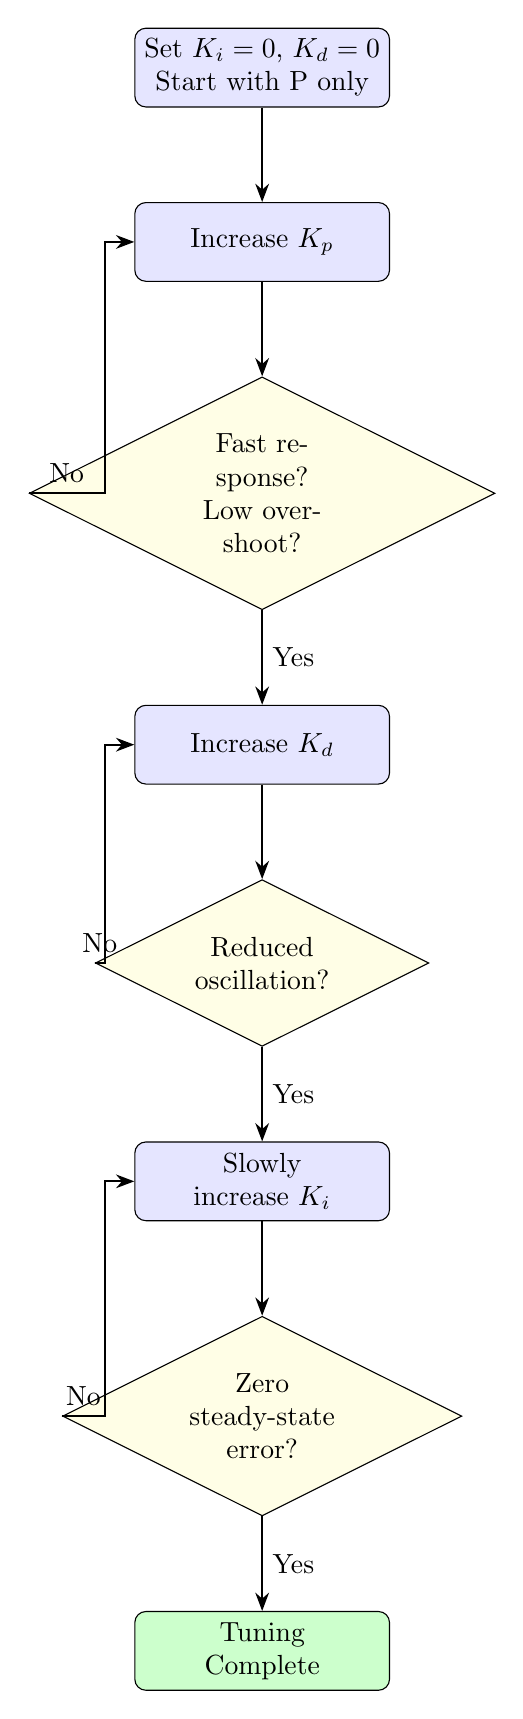
\begin{tikzpicture}[
    node distance=1.2cm and 2cm,
    block/.style={rectangle, draw, fill=blue!10, text width=3cm, align=center, minimum height=1cm, rounded corners},
    decision/.style={diamond, draw, fill=yellow!10, text width=2.2cm, align=center, aspect=2},
    arrow/.style={-Stealth, thick}
]
    % Start
    \node[block] (start) {Set $K_i = 0$, $K_d = 0$\\Start with P only};

    % P tuning
    \node[block, below=of start] (p1) {Increase $K_p$};
    \node[decision, below=of p1] (p2) {Fast response?\\Low overshoot?};

    % D tuning
    \node[block, below=of p2] (d1) {Increase $K_d$};
    \node[decision, below=of d1] (d2) {Reduced\\oscillation?};

    % I tuning
    \node[block, below=of d2] (i1) {Slowly\\increase $K_i$};
    \node[decision, below=of i1] (i2) {Zero\\steady-state\\error?};

    % Done
    \node[block, below=of i2, fill=green!20] (done) {Tuning\\Complete};

    % Arrows with yes/no
    \draw[arrow] (start) -- (p1);
    \draw[arrow] (p1) -- (p2);
    \draw[arrow] (p2) -- node[right] {Yes} (d1);
    \draw[arrow] (p2) -| node[near start, above] {No} ++(-2,0) |- (p1);

    \draw[arrow] (d1) -- (d2);
    \draw[arrow] (d2) -- node[right] {Yes} (i1);
    \draw[arrow] (d2) -| node[near start, above] {No} ++(-2,0) |- (d1);

    \draw[arrow] (i1) -- (i2);
    \draw[arrow] (i2) -- node[right] {Yes} (done);
    \draw[arrow] (i2) -| node[near start, above] {No} ++(-2,0) |- (i1);

\end{tikzpicture}
\caption{PID tuning flowchart. Sequential tuning of P, D, and I gains ensures systematic convergence to stable, responsive control.}
\label{fig:pid_tuning}
\end{figure}

For typical RC aircraft:
\begin{itemize}[noitemsep]
    \item Roll: $K_p \approx 0.5$, $K_i \approx 0.05$, $K_d \approx 0.1$
    \item Pitch: $K_p \approx 0.8$, $K_i \approx 0.08$, $K_d \approx 0.15$
    \item Yaw: $K_p \approx 0.3$, $K_i \approx 0.03$, $K_d \approx 0.05$
\end{itemize}

% ============================================================================
\section{Level 3: Attitude Control (Outer Loop)}
% ============================================================================

\subsection{Cascaded Architecture}

Level 3 forms the \textbf{outer loop} of a cascaded control structure, with Level 4 as the inner loop. This is the core of dRehmFlight's design \cite{rehm_drehm}:

\begin{equation}
\boxed{\text{Angle error} \xrightarrow{\text{Level 3 PID}} \text{Rate command} \xrightarrow{\text{Level 4 PID}} \text{Surface deflection}}
\end{equation}

The separation of angle and rate control provides \cite{stevens2015, franklin2019}:
\begin{itemize}[noitemsep]
    \item \textbf{Frequency separation}: Angle loop $\sim$50--100 Hz, rate loop $\sim$500--1000 Hz
    \item \textbf{Independent tuning}: Tune fast inner loop first, then slower outer loop
    \item \textbf{Disturbance rejection}: Inner loop rapidly corrects rate disturbances
    \item \textbf{Mode switching}: Can bypass angle control for direct rate mode (acro)
\end{itemize}

\subsection{Euler Angle Representation}

Aircraft attitude is parameterized by three Euler angles (3-2-1 yaw-pitch-roll sequence):

\begin{align}
\phi &: \text{Roll angle (rotation about body x-axis)} \\
\theta &: \text{Pitch angle (rotation about body y-axis)} \\
\psi &: \text{Yaw angle (rotation about body z-axis)}
\end{align}

\textbf{Advantages}:
\begin{itemize}[noitemsep]
    \item Intuitive (directly correspond to aircraft orientation)
    \item Easy visualization
    \item Minimal parameterization (3 DOF)
\end{itemize}

\textbf{Limitation --- Gimbal Lock}:

At $\theta = \pm 90°$ (vertical pitch), roll and yaw become coupled (loss of one DOF). The kinematic equations become singular.

\textbf{Mitigation}:
\begin{equation}
\theta_{\text{safe}} = \text{clamp}(\theta, -85°, +85°)
\end{equation}

For aerobatic flight requiring full $360°$ pitch, use quaternions instead.

\subsection{Euler Angle Kinematics}

The relationship between Euler angle rates and body angular rates is:

\begin{equation}
\begin{bmatrix} \dot{\phi} \\ \dot{\theta} \\ \dot{\psi} \end{bmatrix} =
\begin{bmatrix}
1 & \sin\phi \tan\theta & \cos\phi \tan\theta \\
0 & \cos\phi & -\sin\phi \\
0 & \sin\phi / \cos\theta & \cos\phi / \cos\theta
\end{bmatrix}
\begin{bmatrix} p \\ q \\ r \end{bmatrix}
\label{eq:euler_kinematics}
\end{equation}

Inverting Eq.~\eqref{eq:euler_kinematics} (assuming $|\theta| < 85°$) gives the body rates in terms of Euler rates:

\begin{equation}
\begin{bmatrix} p \\ q \\ r \end{bmatrix} =
\begin{bmatrix}
1 & 0 & -\sin\theta \\
0 & \cos\phi & \sin\phi\cos\theta \\
0 & -\sin\phi & \cos\phi\cos\theta
\end{bmatrix}
\begin{bmatrix} \dot{\phi} \\ \dot{\theta} \\ \dot{\psi} \end{bmatrix}
\label{eq:euler_inverse}
\end{equation}

Explicitly:
\begin{align}
p &= \dot{\phi} - \dot{\psi}\sin\theta \\
q &= \dot{\theta}\cos\phi + \dot{\psi}\sin\phi\cos\theta \\
r &= -\dot{\theta}\sin\phi + \dot{\psi}\cos\phi\cos\theta
\end{align}

For small angles ($\phi, \theta \ll 1$ rad) AND small cross-axis rates:

\begin{align}
\dot{\phi} &\approx p \quad \text{(valid if } q\sin\phi\tan\theta \ll p \text{ and } r\cos\phi\tan\theta \ll p \text{)} \nonumber \\
\dot{\theta} &\approx q \quad \text{(valid if } r\sin\phi \ll q \text{)} \nonumber \\
\dot{\psi} &\approx r \quad \text{(valid if } q\sin\phi/\cos\theta \ll r \text{ and } r\cos\phi/\cos\theta \approx r \text{)}
\label{eq:small_angle_approx}
\end{align}

\textbf{Critical clarification:} This approximation requires BOTH:
\begin{enumerate}[noitemsep]
    \item Small Euler angles: $|\phi|, |\theta| < 15°$ (so $\sin\phi \approx \phi$, $\tan\theta \approx \theta$)
    \item Small cross-axis angular rates relative to primary rates
\end{enumerate}

The approximation is \textit{not} valid if angles are small but rates are large (e.g., small roll angle but high pitch/yaw rates), or during coordinated maneuvers where all three rates are significant simultaneously.

\textbf{Application:} This approximation is reasonable for small attitude excursions from level flight (e.g., $|\phi| < 10°$, $|\theta| < 5°$) with gentle maneuvers. For aggressive flight or aerobatics, use the full kinematic equations~\eqref{eq:euler_kinematics}.

\subsection{Cascaded Attitude Controller Design}

The Level 3 controller implements PID on attitude angles, outputting rate commands for Level 4.

\textbf{Roll controller}:

\begin{equation}
p_{cmd}(t) = K_{p,\phi} (\phi_{cmd} - \phi) + K_{i,\phi} \int (\phi_{cmd} - \phi) dt + K_{d,\phi} \frac{d(\phi_{cmd} - \phi)}{dt}
\label{eq:roll_attitude_pid}
\end{equation}

Simplifying (assuming $\dot{\phi}_{cmd} \approx 0$ for setpoint tracking):

\begin{equation}
p_{cmd} = K_{p,\phi} e_\phi + K_{i,\phi} \int e_\phi dt - K_{d,\phi} \dot{\phi}
\end{equation}

where $e_\phi = \phi_{cmd} - \phi$.

Using the small-angle approximation $\dot{\phi} \approx p$:

\begin{equation}
p_{cmd} = K_{p,\phi} e_\phi + K_{i,\phi} \int e_\phi dt - K_{d,\phi} p
\label{eq:roll_with_rate_feedback}
\end{equation}

\textbf{Derivative-on-measurement technique:}

This formulation uses $-K_d p$ instead of $+K_d \dot{e}_\phi$ (derivative of error). This is called \textbf{derivative-on-measurement} or \textbf{rate feedback}, and it provides important advantages:

\begin{enumerate}[noitemsep]
    \item \textbf{Cleaner signal}: Angular rates $p, q, r$ come directly from gyroscopes (clean, high-bandwidth measurements), whereas differentiating Euler angles amplifies sensor noise and quantization
    \item \textbf{No derivative kick}: When the setpoint $\phi_{cmd}$ changes suddenly (step command), $\dot{e}_\phi$ has a spike, causing unwanted control transients. Using $-K_d p$ avoids this because $p$ changes smoothly
    \item \textbf{Equivalent damping}: For setpoint tracking with slowly-varying commands, $\dot{e}_\phi \approx -\dot{\phi} \approx -p$, so the two formulations are equivalent in steady-state
\end{enumerate}

\textbf{Important distinction:} The effective derivative gain differs from pure error derivative. With derivative-on-measurement, we're damping the \textit{output} (rate) rather than the error derivative. This is superior for cascaded control where the inner loop directly measures rates.

This is a PD controller on angle error with integral correction, using current rate $p$ as derivative feedback.

Similarly for pitch and yaw:

\begin{align}
q_{cmd} &= K_{p,\theta} e_\theta + K_{i,\theta} \int e_\theta dt - K_{d,\theta} q \\
r_{cmd} &= K_{p,\psi} e_\psi + K_{i,\psi} \int e_\psi dt - K_{d,\psi} r
\end{align}

\textbf{Rate limiting}:

Rate commands must be within achievable limits:

\begin{align}
p_{cmd} &\in [-p_{\max}, +p_{\max}], \quad \text{typically } p_{\max} = 180°/\text{s} \\
q_{cmd} &\in [-q_{\max}, +q_{\max}], \quad \text{typically } q_{\max} = 180°/\text{s} \\
r_{cmd} &\in [-r_{\max}, +r_{\max}], \quad \text{typically } r_{\max} = 90°/\text{s}
\end{align}

\subsection{Gain Tuning for Attitude Controllers}

The \textbf{inner loop (Level 4) must be tuned first}, then the outer loop (Level 3). This ensures the inner loop is fast and tight before the outer loop commands it.

\textbf{Frequency separation rule}:

\begin{equation}
\omega_{\text{outer}} \leq \frac{1}{10} \omega_{\text{inner}}
\end{equation}

If the inner loop has 10 Hz bandwidth, the outer loop should have $\leq 1$ Hz bandwidth.

\textbf{Outer loop tuning}:

\begin{itemize}[noitemsep]
    \item Start with $K_i = 0$, $K_d = 0$
    \item Increase $K_p$ until response is smooth with $\sim$10\% overshoot
    \item Add $K_d$ to reduce overshoot (typically $K_d \approx 0.05 K_p$ for outer loop)
    \item Add $K_i$ sparingly to eliminate offset (typically $K_i \approx 0.01 K_p$)
\end{itemize}

Typical values for RC aircraft:
\begin{itemize}[noitemsep]
    \item Roll angle: $K_p \approx 5.0$, $K_i \approx 0.5$, $K_d \approx 0.3$
    \item Pitch angle: $K_p \approx 6.0$, $K_i \approx 0.6$, $K_d \approx 0.4$
    \item Yaw angle: $K_p \approx 3.0$, $K_i \approx 0.3$, $K_d \approx 0.2$
\end{itemize}

% ============================================================================
\section{Level 2: HSA Control}
% ============================================================================

\subsection{Flight State Variables}

Level 2 controls three flight state variables:

\begin{itemize}[noitemsep]
    \item \textbf{Heading (H)}: $\psi$ (rad), compass direction (0 = North, $\pi/2$ = East)
    \item \textbf{Speed (S)}: $V$ (m/s), airspeed magnitude
    \item \textbf{Altitude (A)}: $h$ (m), height above reference
\end{itemize}

These are the primary variables for autonomous flight missions.

\subsection{HSA to Attitude Mapping}

Level 2 converts HSA commands to attitude commands for Level 3.

\subsubsection{Heading Control via Coordinated Turn}

To change heading, the aircraft must bank (roll) and turn. For a coordinated turn (zero sideslip), the required bank angle is:

\begin{equation}
\phi_{cmd} = \arctan\left(\frac{V^2}{g R}\right) = \arctan\left(\frac{V \dot{\psi}}{g}\right)
\label{eq:coordinated_turn_exact}
\end{equation}

where $R$ is turn radius, $g = 9.81$ m/s$^2$, and $\dot{\psi} = V/R$ for circular motion.

\textbf{Small-angle approximation:} For small bank angles ($|\phi| < 15°$, so $\arctan(\phi) \approx \phi$):

\begin{equation}
\phi_{cmd} \approx \frac{V \dot{\psi}}{g}
\label{eq:coordinated_turn}
\end{equation}

This approximation is valid when $V\dot{\psi}/g < 0.26$ (corresponding to $\phi < 15°$). For tighter turns or higher speeds, use the exact arctangent formulation Eq.~\eqref{eq:coordinated_turn_exact}.

A PID controller on heading error produces yaw rate, which maps to roll angle:

\begin{align}
\psi_{\text{error}} &= \psi_{cmd} - \psi \quad \text{(wrapped to } [-\pi, \pi]) \\
r_{\text{des}} &= K_{p,H} \psi_{\text{error}} \\
\phi_{cmd} &= K_{\phi r} r_{\text{des}} \quad \text{(typically } K_{\phi r} \approx 0.5 \text{)}
\end{align}

\subsubsection{Altitude Control via Pitch}

Altitude error drives climb rate, which maps to pitch angle via the climb equation.

\textbf{Physical relationship:} For small angles and moderate speeds, the climb rate is:
\begin{equation}
\dot{h} \approx V \sin(\theta - \alpha) \approx V(\theta - \alpha)
\label{eq:climb_rate}
\end{equation}

where $\alpha$ is angle of attack (typically $\alpha_{\text{trim}} \approx 2°$--$5°$ in cruise).

Solving for pitch angle:
\begin{equation}
\theta_{cmd} = \alpha_{\text{trim}} + \frac{\dot{h}_{\text{des}}}{V}
\label{eq:pitch_from_climb}
\end{equation}

\textbf{Implementation:}

\begin{align}
h_{\text{error}} &= h_{cmd} - h \\
\dot{h}_{\text{des}} &= K_{p,A} h_{\text{error}} \quad \text{(clamped to } \pm 5 \text{ m/s)} \\
\theta_{cmd} &= \alpha_{\text{trim}} + \frac{\dot{h}_{\text{des}}}{V_{\text{safe}}}
\end{align}

where $V_{\text{safe}} = \max(V, 15~\text{m/s})$ prevents excessive pitch commands at low airspeed, and $\alpha_{\text{trim}}$ is the trim angle of attack (can be set to zero for simplicity, or estimated as $\alpha_{\text{trim}} \approx 3°$).

\textbf{Alternative empirical mapping:} If the physical relationship is unknown or airspeed is not available, an empirical gain can be used:
\begin{equation}
\theta_{cmd} \approx K_{h\theta} \dot{h}_{\text{des}} \quad \text{where } K_{h\theta} \approx \frac{1}{V_{\text{cruise}}} \text{ [rad·s/m]}
\end{equation}

The physically-based formulation Eq.~\eqref{eq:pitch_from_climb} is preferred as it automatically adapts to airspeed variations.

\subsubsection{Speed Control via Throttle}

Speed error maps directly to throttle:

\begin{align}
V_{\text{error}} &= V_{cmd} - V \\
\delta_t &= \delta_{t,\text{baseline}} + K_{p,S} V_{\text{error}} + K_{i,S} \int V_{\text{error}} dt
\end{align}

where $\delta_{t,\text{baseline}} \approx 0.5$ is cruise throttle.

\subsection{HSA Controller Architecture}

The complete Level 2 controller:

\begin{algorithm}[H]
\caption{HSA Control Loop (10--50 Hz)}
\begin{algorithmic}[1]
\State \textbf{Input}: $\psi_{cmd}, V_{cmd}, h_{cmd}$, current state
\State \textbf{Output}: $\phi_{cmd}, \theta_{cmd}, \psi_{cmd}, \delta_t$
\State
\State $\psi_{\text{error}} \gets$ wrap$(\psi_{cmd} - \psi)$
\State $\phi_{cmd} \gets$ HeadingPID$(\psi_{\text{error}})$ \Comment{Maps to roll}
\State
\State $h_{\text{error}} \gets h_{cmd} - h$
\State $\theta_{cmd} \gets$ AltitudePID$(h_{\text{error}})$ \Comment{Maps to pitch}
\State
\State $V_{\text{error}} \gets V_{cmd} - V$
\State $\delta_t \gets$ SpeedPID$(V_{\text{error}})$ \Comment{Throttle}
\State
\State Send $(\phi_{cmd}, \theta_{cmd}, \psi_{cmd}, \delta_t)$ to Level 3
\end{algorithmic}
\end{algorithm}

% ============================================================================
\section{Level 1: Waypoint Navigation}
% ============================================================================

\subsection{Guidance Algorithms}

Level 1 converts 3D waypoint positions to HSA commands using guidance algorithms.

\subsubsection{Line-of-Sight (LOS) Guidance}

The simplest guidance law: point directly at the waypoint.

Given current position $\vect{p}_{\text{curr}} = [N, E, D]^T$ and waypoint $\vect{p}_{\text{wp}} = [N_{\text{wp}}, E_{\text{wp}}, D_{\text{wp}}]^T$:

\begin{align}
\Delta N &= N_{\text{wp}} - N \\
\Delta E &= E_{\text{wp}} - E \\
\psi_{cmd} &= \text{atan2}(\Delta E, \Delta N) \label{eq:los_heading} \\
h_{cmd} &= -D_{\text{wp}} \quad \text{(altitude positive up)} \\
V_{cmd} &= V_{\text{cruise}} \quad \text{(or waypoint-specified speed)}
\end{align}

\textbf{Waypoint acceptance}: Declare waypoint reached when:

\begin{equation}
\sqrt{(\Delta N)^2 + (\Delta E)^2 + (\Delta D)^2} < R_{\text{accept}}
\end{equation}

where typically $R_{\text{accept}} = 10$ m.

\subsubsection{Proportional Navigation (Advanced)}

For more aggressive pursuit, proportional navigation commands acceleration perpendicular to line-of-sight:

\begin{equation}
\vect{a}_{\perp} = N' V_{\text{closing}} \dot{\vect{\lambda}}
\end{equation}

where $N' \in [3,5]$ is navigation constant, $V_{\text{closing}}$ is closing velocity, and $\dot{\vect{\lambda}}$ is line-of-sight rate.

This is more complex but provides tighter tracking of moving targets.

% ============================================================================
\section{Level 5: Direct Surface Control}
% ============================================================================

Level 5 is direct surface actuation, primarily for:
\begin{itemize}[noitemsep]
    \item Reinforcement learning research (learn from scratch)
    \item Novel aircraft configurations (no established control laws)
    \item Control allocation optimization
\end{itemize}

At this level, the agent directly commands $\delta_a, \delta_e, \delta_r, \delta_t \in [-1,1]$, which are mapped to actuator commands (e.g., servo PWM signals).

This is the lowest abstraction, offering maximum control authority but requiring the agent to understand full aircraft dynamics.

% ============================================================================
\section{Mathematical Foundations}
% ============================================================================

\subsection{Frequency Domain Analysis}

Cascaded control stability relies on frequency separation. In the Laplace domain, the closed-loop transfer function of the cascaded system is:

\begin{equation}
G_{\text{cascade}}(s) = \frac{G_{\text{outer}}(s) G_{\text{inner}}(s)}{1 + G_{\text{inner}}(s) H_{\text{inner}}(s)} \cdot \frac{1}{1 + G_{\text{outer}}(s) H_{\text{outer}}(s)}
\end{equation}

If the inner loop bandwidth $\omega_{\text{inner}} \gg \omega_{\text{outer}}$, the loops decouple and can be designed independently.

\textbf{Bode plot criterion}: The inner loop crossover frequency should be $10\times$ higher than the outer loop for clean separation.

\subsection{Stability via Small Gain Theorem}

For cascaded loops, the small gain theorem ensures stability if each loop is individually stable and coupling is weak:

\begin{equation}
\|G_{\text{coupling}}\|_\infty < \frac{1}{\|G_{\text{loop}}\|_\infty}
\end{equation}

This justifies the decoupled multi-axis design.

% ============================================================================
\section{Implementation Details}
% ============================================================================

\subsection{Software Architecture}

The control hierarchy is implemented as a hybrid Python/C++ system:

\begin{itemize}[noitemsep]
    \item \textbf{Levels 1--3}: Python (flexibility for research, RL integration)
    \item \textbf{Levels 4--5}: C++ (performance for high-frequency control)
    \item \textbf{Interface}: Pybind11 for zero-copy data transfer
\end{itemize}

\textbf{File structure}:
\begin{lstlisting}
controllers/
  base_agent.py           # Abstract agent interface
  rate_agent.py           # Level 4 (Python wrapper)
  attitude_agent.py       # Level 3 (cascaded outer loop)
  hsa_agent.py            # Level 2
  waypoint_agent.py       # Level 1

cpp/
  src/pid_controller.cpp  # C++ PID implementation
  bindings/bindings.cpp   # Pybind11 interface
\end{lstlisting}

\subsection{Real-Time Execution}

Control loops run at different priorities:

\begin{table}[H]
\centering
\caption{Thread Priorities and Timing}
\begin{tabular}{|l|c|c|c|}
\hline
\textbf{Thread} & \textbf{Frequency} & \textbf{Priority} & \textbf{Latency Budget} \\
\hline
Level 4 (C++) & 1000 Hz & Highest & < 1 ms \\
Level 3 (C++) & 100 Hz & High & < 10 ms \\
Level 2 (Python) & 50 Hz & Medium & < 20 ms \\
Level 1 (Python) & 10 Hz & Low & < 100 ms \\
Logging & Async & Lowest & Best-effort \\
\hline
\end{tabular}
\end{table}

% ============================================================================
\section{Comparison to Industry Standards}
% ============================================================================

\subsection{dRehmFlight Architecture}

dRehmFlight \cite{rehm_drehm} implements a two-loop cascaded structure:

\begin{itemize}[noitemsep]
    \item \textbf{Angle mode}: Outer PID on Euler angles → rate commands
    \item \textbf{Rate mode}: Inner PID on angular rates → surface deflections
\end{itemize}

This is exactly our Levels 3--4. We extend dRehmFlight by adding:
\begin{itemize}[noitemsep]
    \item Level 2 (HSA) for autonomous flight
    \item Level 1 (Waypoint) for mission planning
    \item Level 5 (explicit surface layer) for RL research
\end{itemize}

\subsection{Comparison Table}

\begin{table}[H]
\centering
\caption{Control Architecture Comparison}
\label{tab:comparison}
\begin{tabular}{|l|c|c|c|}
\hline
\textbf{Feature} & \textbf{dRehmFlight} & \textbf{Betaflight} & \textbf{This Work} \\
\hline
Angle mode & \checkmark & \checkmark & \checkmark (L3) \\
Rate mode & \checkmark & \checkmark & \checkmark (L4) \\
HSA control & -- & Limited & \checkmark (L2) \\
Waypoint nav & -- & -- & \checkmark (L1) \\
Language & C++ & C & Python + C++ \\
Loop rate (inner) & 500 Hz & 8000 Hz & 1000 Hz \\
Loop rate (outer) & 100 Hz & 500 Hz & 100 Hz \\
License & GPL v3 & GPL v3 & (Project-specific) \\
\hline
\end{tabular}
\end{table}

\textbf{Acknowledgment}: Our core cascaded design (Levels 3--4) is directly inspired by and follows the proven architecture of dRehmFlight.

% ============================================================================
\section{Conclusion}
% ============================================================================

This document has presented a comprehensive five-level hierarchical control architecture for fixed-wing aircraft, combining the proven cascaded angle-rate structure of dRehmFlight with additional high-level layers for autonomous flight and reinforcement learning research.

\textbf{Key contributions}:
\begin{enumerate}[noitemsep]
    \item Rigorous mathematical foundations for each control level
    \item Extension of dRehmFlight's two-loop design to five levels
    \item Detailed implementation guidance (C++ and Python)
    \item Comparison to industry-standard flight controllers
    \item Suitability for both simulation and hardware deployment
\end{enumerate}

\textbf{Acknowledgments}: This architecture owes a significant intellectual debt to Nicholas Rehm's dRehmFlight project, which established the clean separation between angle and rate control that forms the foundation of modern flight controllers. We gratefully acknowledge this inspiration while noting that our implementation is original work.

The five-level architecture provides flexibility for researchers and practitioners to choose the appropriate abstraction level for their application, from high-level mission planning down to low-level surface optimization.

% ============================================================================
% References
% ============================================================================
\begin{thebibliography}{9}

\bibitem{rehm_drehm}
Rehm, Nicholas (2020).
\textit{dRehmFlight: Teensy Flight Controller for VTOL Aircraft.}
GitHub repository.
\url{https://github.com/nickrehm/dRehmFlight}.
Licensed under GNU GPL v3.0.

\bibitem{betaflight}
Betaflight Contributors (2023).
\textit{Betaflight: Open Source Flight Controller Firmware.}
\url{https://github.com/betaflight/betaflight}.

\bibitem{ardupilot}
ArduPilot Development Team (2023).
\textit{ArduPilot: Open Source Autopilot Software.}
\url{https://ardupilot.org}.

\bibitem{px4}
PX4 Development Team (2023).
\textit{PX4 Autopilot: Professional Autopilot.}
\url{https://px4.io}.

\bibitem{stevens2015}
Stevens, B. L., Lewis, F. L., \& Johnson, E. N. (2015).
\textit{Aircraft Control and Simulation: Dynamics, Controls Design, and Autonomous Systems} (3rd ed.).
John Wiley \& Sons.

\bibitem{etkin2005}
Etkin, B., \& Reid, L. D. (2005).
\textit{Dynamics of Flight: Stability and Control} (3rd ed.).
John Wiley \& Sons.

\bibitem{nelson1998}
Nelson, R. C. (1998).
\textit{Flight Stability and Automatic Control} (2nd ed.).
McGraw-Hill.

\bibitem{astrom2006}
Åström, K. J., \& Hägglund, T. (2006).
\textit{Advanced PID Control}.
ISA-The Instrumentation, Systems, and Automation Society.

\bibitem{franklin2019}
Franklin, G. F., Powell, J. D., \& Emami-Naeini, A. (2019).
\textit{Feedback Control of Dynamic Systems} (8th ed.).
Pearson.

\end{thebibliography}

\end{document}
